% \subsection{Integration der KI-Tools}

\subsection{Demonstration mit GitHub Copilot}

\subsubsection{Setup und Vorgehen}
Die Entwicklung des Map-Screens wurde exemplarisch mit \textbf{GitHub Copilot}
in Visual Studio Code durchgeführt. Für größtmögliche Vergleichbarkeit kamen
ausschließlich die Copilot-Funktionen zum Einsatz, keine weiteren KI-Plugins.
Ziel war die Umsetzung eines Map-Screens mit Event-Markern, Filterfunktion
sowie Detailansicht – sämtliche Eventdaten stammen dabei aus dem zentralen
EventsProvider.

\begin{figure}[htbp]
      \centering
      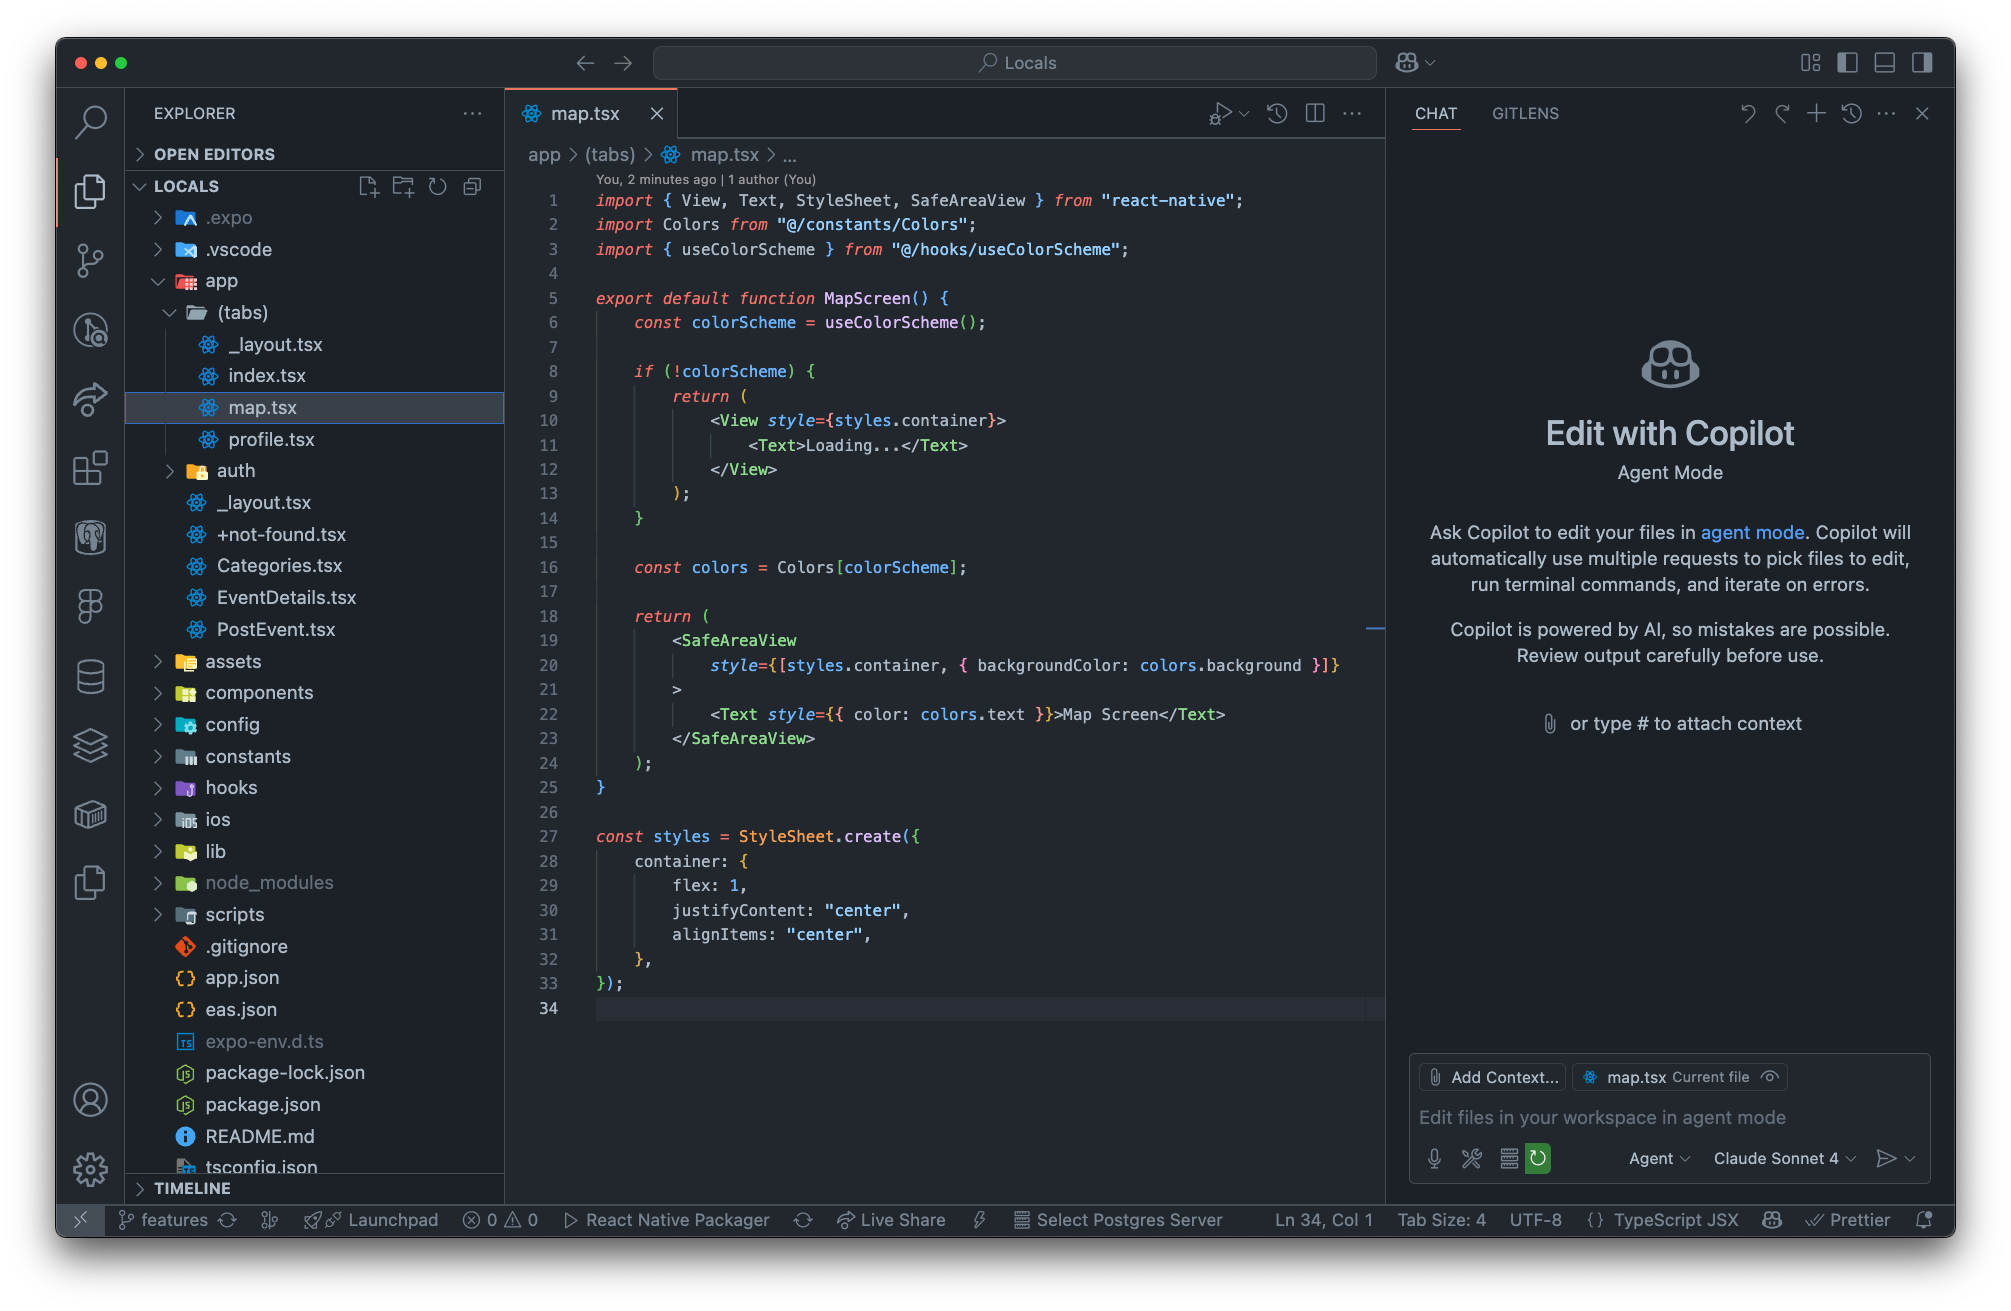
\includegraphics[width=0.95\textwidth]{images/copilot_screenshots/Screenshots Ist-Zustand-copilot.png}
      \caption{Ausgangszustand der Anwendung vor dem Einsatz von Copilot. \textit{Copilot-Demo}}
      \label{fig:copilot-istzustand}
\end{figure}

Vor Beginn der Implementierung wurde Copilot aktiviert und die
Entwicklungsumgebung vorbereitet (z.~B.\ Installation von
\texttt{react-native-maps} und \texttt{expo-location}). Die Aufgabenstellung
für Copilot wurde jeweils als präziser Kommentar oder Docstring formuliert.
Beispielsweise:

\begin{lstlisting}[language=HTML]
// Create a React Native component for a map with event markers and filter functionality
\end{lstlisting}

Oder als umfangreicher Prompt:
\begin{lstlisting}[language=HTML]
// Create a Map Screen with Event Markers and Filter in React Native. Requirements:
//
// - Use event data from the EventsProvider context
// - Show markers, enable filtering, display event details in modal/callout
// - Clean, modular, and maintainable code, with modern UI/UX
\end{lstlisting}

% \begin{figure}[htbp]
%       \centering
%       \includegraphics[width=0.55\textwidth]{images/copilot_screenshots/rückmeldung nach 1. prompt eingabe-copilot.png}
%       \caption{Reaktion von GitHub Copilot auf den ersten Prompt zur Implementierung des MapScreens. \textit{Copilot-Demo}}
%       \label{fig:copilot-erster-prompt}
% \end{figure}

\begin{figure}[htbp]
      \centering
      \begin{minipage}{0.48\textwidth}
            \centering
            \includegraphics[width=0.98\textwidth]{images/copilot_screenshots/implementation-rückmeldung-copilot-1.png}
            \caption{Rückmeldung von Copilot – Teil 1.}
            \label{fig:copilot-impl1}
      \end{minipage}
      \hfill
      \begin{minipage}{0.48\textwidth}
            \centering
            \includegraphics[width=0.98\textwidth]{images/copilot_screenshots/implementation-rückmeldung-copilot-2.png}
            \caption{Rückmeldung von Copilot – Teil 2.}
            \label{fig:copilot-impl2}
      \end{minipage}
      \caption{Schrittweise Rückmeldung und Hinweise von Copilot während der Implementierung. \textit{Eigene Screenshots}}
      \label{fig:copilot-impl-pair}
\end{figure}

\subsubsection{Schrittweise Umsetzung und Reflexion}

Die Entwicklung erfolgte nach folgendem Muster:
\begin{enumerate}
      \item \textbf{Prompt definieren:} Pro Feature (z.\,B. Marker, Filter, Event-Details) wurde ein spezifischer Kommentar als Arbeitsanweisung eingefügt.
      \item \textbf{Vorschläge von Copilot akzeptieren oder anpassen:} Vorschläge wurden Schritt für Schritt übernommen, angepasst oder verworfen.
      \item \textbf{Test und Dokumentation:} Nach jeder Änderung wurde der Code getestet und die Funktionsweise reflektiert.
      \item \textbf{Fehlersuche und Nacharbeit:} Fehlerhafte Vorschläge oder Bugs wurden nach Rücksprache mit Copilot, durch Google-Suche oder manuelle Nacharbeit behoben.
\end{enumerate}

\textbf{Beispiel:}
Zur Erstellung des MapScreens wurde folgender Prompt verwendet (gekürzt):

\begin{lstlisting}[language=HTML]
// Create a React Native component called `MapScreen` that displays event markers on a map using event data from the `EventsProvider` context. Requirements:
//
// - Show all events as markers on a map
// - When a marker is tapped, show details
// - Add filter options above the map
// - Handle loading/error states appropriately
\end{lstlisting}

Die technische Umsetzung umfasste:
\begin{itemize}
      \item Anzeige aller Events als Marker (mit Kategorie und Titel) auf der Karte
            (\texttt{react-native-maps}).
      \item Umsetzung einer Filterleiste zur Auswahl nach Kategorie und Datum.
      \item Darstellung von Event-Details beim Tippen auf einen Marker (Callout oder
            Modal).
      \item Responsives Layout und modernes UI-Design nach Vorgabe.
      \item Fehler- und Ladezustände wurden entsprechend behandelt.
\end{itemize}

\begin{figure}[htbp]
      \centering
      \begin{minipage}{0.48\textwidth}
            \centering
            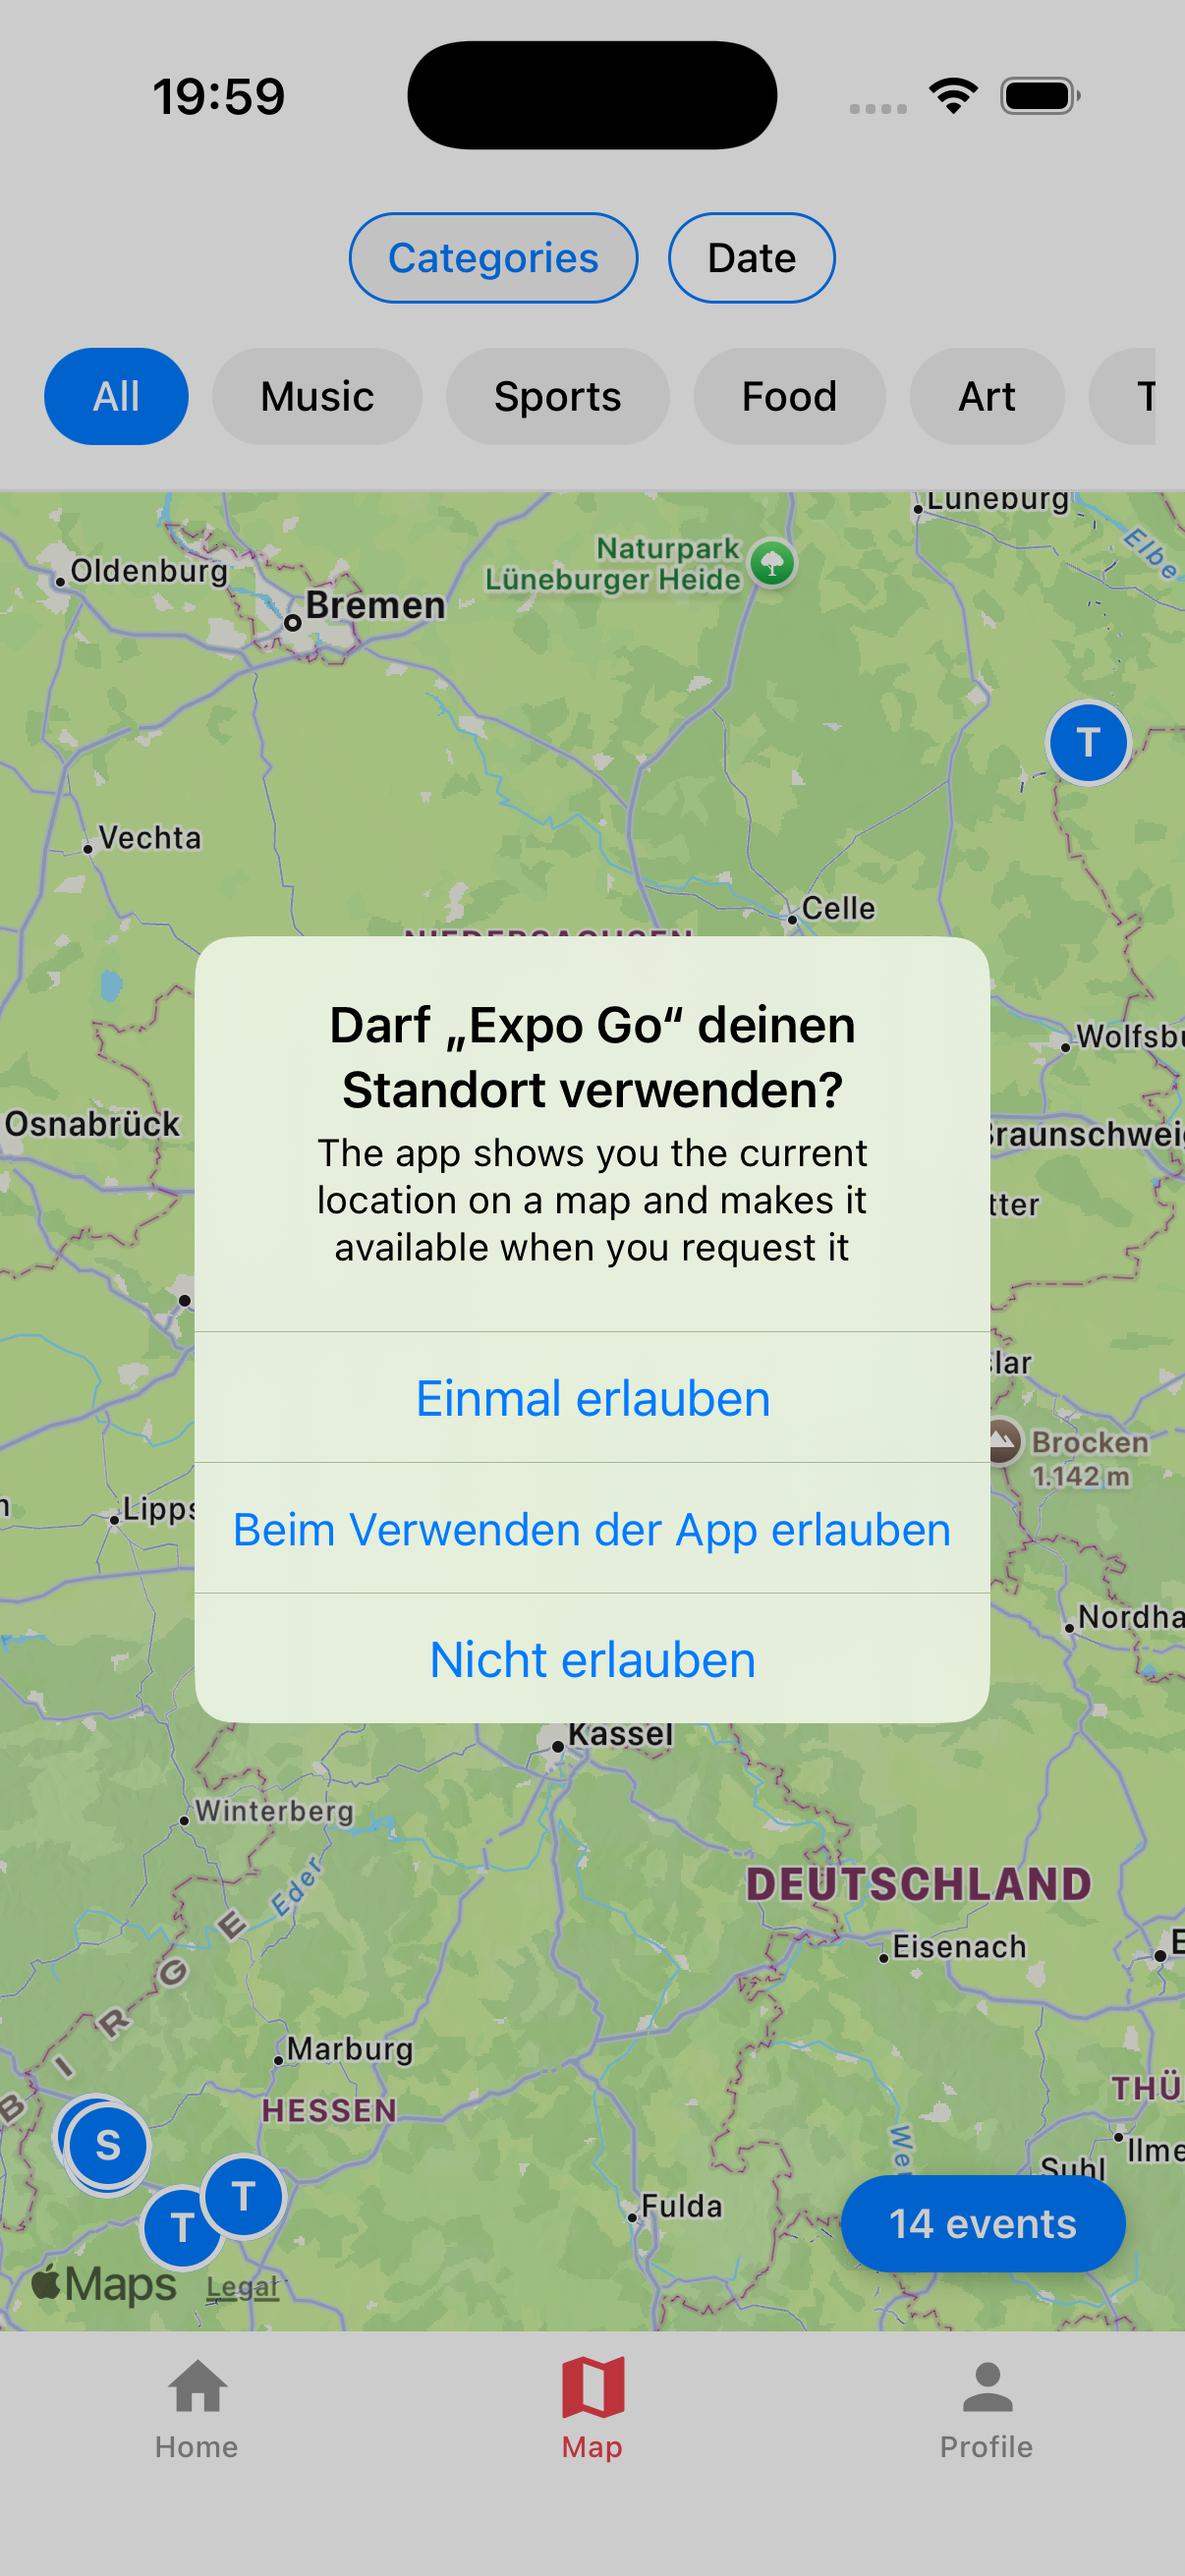
\includegraphics[width=\textwidth]{images/copilot_screenshots/6. 1. Version das MapScreens - Screenshot-copilot.png}
            \caption{Erste lauffähige Version des MapScreens nach KI-gestützter Entwicklung.}
      \end{minipage}
      \hfill
      \begin{minipage}{0.48\textwidth}
            \centering
            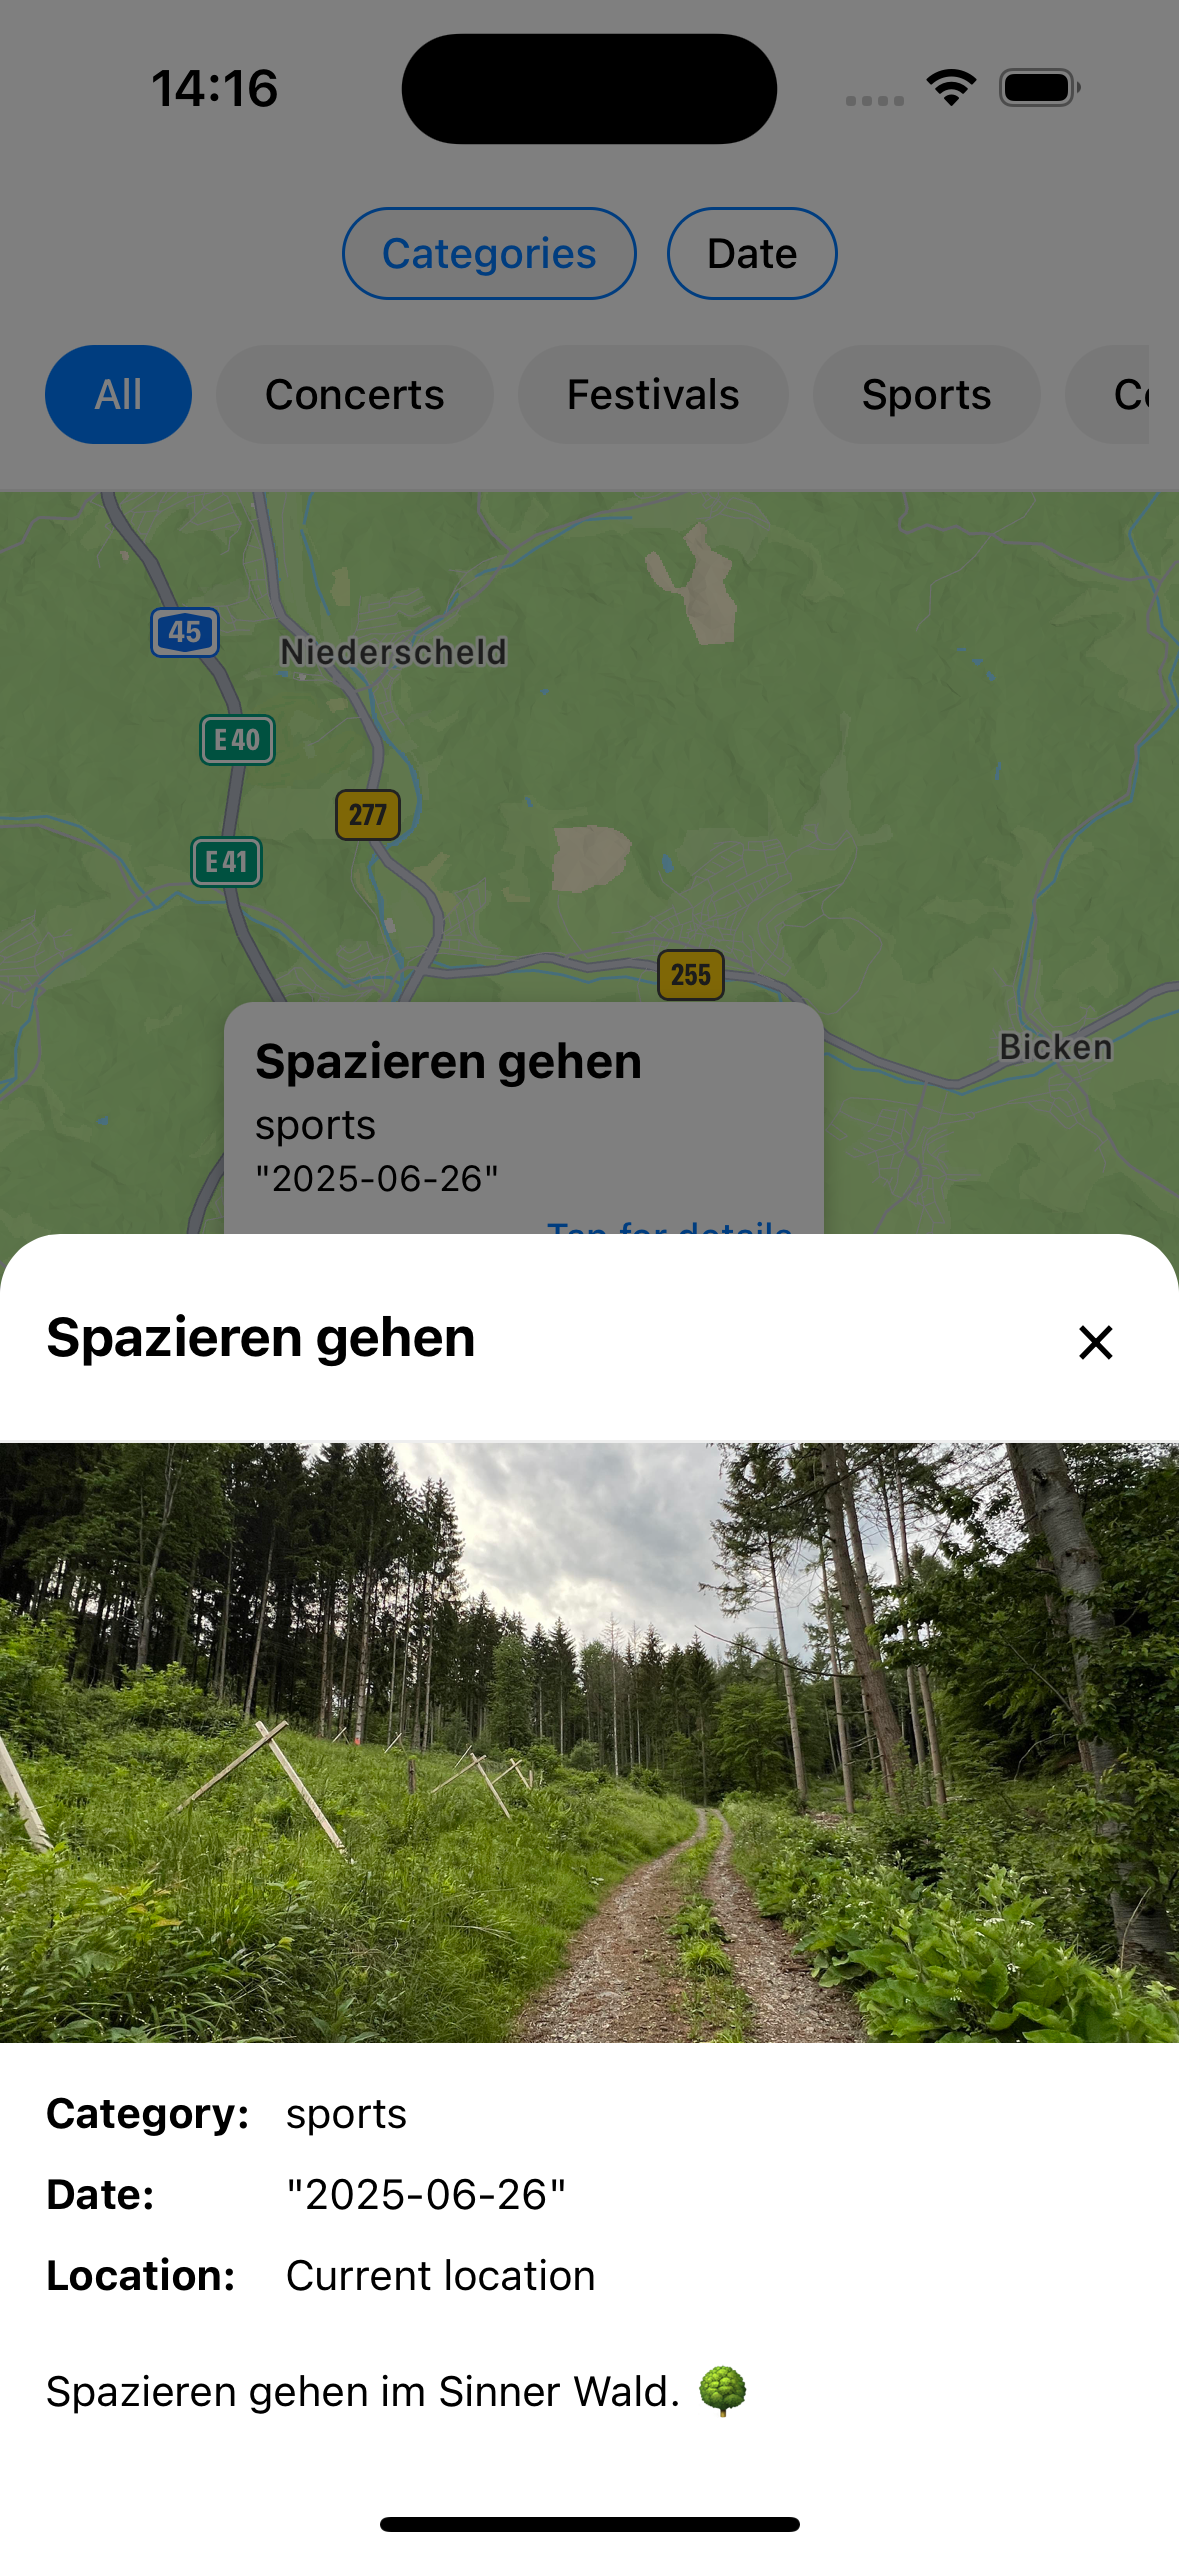
\includegraphics[width=\textwidth]{images/copilot_screenshots/Callouts+modal-copilot.png}
            \caption{Event-Details und Callouts auf dem MapScreen.}
            \label{fig:copilot-callouts}
      \end{minipage}
\end{figure}

Die Code-Generierung erfolgte modular und meist nachvollziehbar. Beispiel:
Copilot erstellte automatisch das Grundgerüst einer Map-Komponente, ergänzte
dann Schritt für Schritt die Logik für Marker, Filter und Event-Details.

Die in dieser Arbeit beobachteten Stärken und Schwächen von GitHub Copilot
decken sich mit den Ergebnissen anderer Studien. So berichtet
Kerr~\cite{kerr_github_nodate}, dass Copilot die Entwicklung von
React-Anwendungen deutlich beschleunigen kann, jedoch eine kritische
Überprüfung der Vorschläge unerlässlich bleibt. Weisz
et~al.~\cite{weisz_design_2024} betonen zudem, dass die Gestaltung der
Interaktion und Feedbackmechanismen einen maßgeblichen Einfluss auf die
Akzeptanz der KI-gestützten Codegenerierung hat.

\subsubsection{Herausforderungen und Beobachtungen}
Im Verlauf der Entwicklung zeigte Copilot verschiedene Stärken und Schwächen:

\textbf{Stärken:}
\begin{itemize}
      \item Effiziente Generierung von Boilerplate-Code und wiederkehrenden Patterns
            (z.\,B. Hook-Nutzung, State-Management).
      \item Schnelle Vorschläge für UI-Komponenten und einfache Interaktionslogik.
      \item Erkennung von einfachen Fehlern und automatische Typanpassung nach Änderungen
            (z.\,B. bei Änderung der Datenstruktur für Kategorien).
\end{itemize}

\textbf{Schwächen und typische Fehlerquellen:}
\begin{itemize}
      \item Teilweise fehlerhafte oder veraltete Import-Pfade (z.\,B. bei Kategorien).
      \item Missverständnisse bei nicht exakt spezifizierten Datenstrukturen (z.\,B.
            Umwandlung von Kategorien-Array von String zu Objekt wurde erst nach manuellem
            Eingriff korrekt erkannt).
      \item Filter-Logik für den ``All''-Filter funktionierte zunächst nicht wie erwartet;
            Copilot schlug Anpassungen vor, die jedoch neue Fehler erzeugten (zwei
            ``All''-Filter, Duplicate-Key-Warning).
      \item In mehreren Iterationen blieb die Korrektur von Spezialfällen (wie
            Filter-Probleme oder Typkonflikte) hinter den Erwartungen zurück, sodass
            letztlich manuelle Nachbesserung notwendig wurde.
\end{itemize}

\textbf{Reflexion:}
\begin{itemize}
      \item Die Vorschläge waren bei Standardaufgaben meist brauchbar (\textit{Subjektive
                  Zufriedenheit: 4/5}), bei komplexeren State- oder Typ-Logiken aber oft
            unvollständig.
      \item Die Interaktion mit Copilot war intuitiv, erfordert jedoch genaue Prompts und
            ein grundsätzliches Verständnis für die Implementierung, um Fehlerquellen zu
            erkennen und zu korrigieren.
      \item Bei UI-Details oder individuelleren Anforderungen blieb Nacharbeit
            unerlässlich.
\end{itemize}

\textbf{Fazit:}
Copilot ist ein sehr leistungsfähiges Assistenz-Tool, das Routinearbeiten und Standardaufgaben erheblich beschleunigt. Bei komplexeren oder individuelleren Anforderungen stößt es jedoch an Grenzen, sodass eine kritische Prüfung und manuelle Nacharbeit weiterhin unverzichtbar bleibt. Die Demonstration belegt, dass Copilot einen relevanten Effizienzgewinn für erfahrene Entwickler:innen bieten kann, den Anspruch auf vollständige Automatisierung jedoch (noch) nicht erfüllt.

\subsection{Demonstration mit Cursor}

\subsubsection{Setup und Vorgehen}
Für die Entwicklung des Map-Screens wurde \textbf{Cursor} als spezialisierte
KI-basierte Entwicklungsumgebung genutzt (Branch: \texttt{cursor},
Sprachmodell: Claude 3.7 Sonnet, Agent mode). Cursor ermöglicht Prompt
Chaining, die Verarbeitung von Screenshots als Referenz und einen
dialogbasierten Entwicklungsprozess.

Zu Beginn wurden Screenshots des aktuellen App-Zustands sowie relevanter
Komponenten (u.\,a. \texttt{\_layout.tsx}, Event Provider) als Kontext
bereitgestellt. Der Hauptprompt für den Einstieg lautete:

\begin{lstlisting}[language=HTML]
// Create a Map Screen with Event Markers and Filter in React Native. Requirements:
//
// - Use event data from the EventsProvider context
// - Show markers, enable filtering, display event details in modal/callout
// - Clean, modular, and maintainable code, with modern UI/UX 
// - Use provided screenshots/layouts as visual reference
\end{lstlisting}

\subsubsection{Schrittweise Umsetzung und Reflexion}

Der Entwicklungsprozess war durch mehrere Besonderheiten gekennzeichnet:

\begin{enumerate}
      \item \textbf{Prompt Chaining und Screenshot-Kontext:} Zu jedem Entwicklungsschritt wurden gezielt neue Prompts mit aktualisierten Anforderungen und Referenz-Screenshots gestellt.
      \item \textbf{Terminal-Steuerung:} Cursor führte notwendige Terminalbefehle (z.\,B. Paketinstallationen) eigenständig aus und dokumentierte Fehlermeldungen sowie Lösungsvorschläge direkt im Chat.
      \item \textbf{Debugging und Package-Kompatibilität:} Cursor identifizierte eigenständig Kompatibilitätsprobleme, z.\,B. bei der \texttt{react-native-maps}-Version (\^1.24.3 statt \^1.18.0), und schlug proaktiv eine Anpassung auf die funktionierende Version vor.
      \item \textbf{Iterative Korrekturen und UX-Verbesserungen:} Bei UI-Problemen (z.\,B. überlagernde Filter/Buttons) wurden nach Rückmeldung gezielt Layout-Vorschläge unterbreitet.
      \item \textbf{Feature-Integration:} Funktionen wie Filter, Refresh-Button und Navigation zu Event-Standorten wurden auf Nachfrage oder eigenständig ergänzt.
\end{enumerate}

\textbf{Besonders positiv fiel auf:}
\begin{itemize}
      \item Cursor war bei der Behebung von Package-Fehlern und bei der automatischen
            Adaption von Code an neue Datenstrukturen (z.\,B. Kategorien als Objekte statt
            Strings) sehr präzise.
      \item Im Vergleich zu Copilot wurde die grundlegende Kartenfunktion schneller
            funktionsfähig, auch wenn die erste Map-Anzeige erst nach mehreren Prompts
            erschien.
      \item Cursor dokumentierte seine Debugging-Schritte transparent und schlug auch
            Lösungen für übersehene Fehlerquellen vor.
\end{itemize}

\subsubsection{Herausforderungen und Learnings}
\begin{itemize}
      \item \textbf{Versionierung und Abhängigkeiten:} Kompatibilitätsprobleme zwischen \texttt{react-native-maps} und Expo führten zu Fehlern, die erst nach mehreren Iterationen und Prompts gelöst wurden.
      \item \textbf{Automatische Code-Generierung:} Cursor wechselte in einem Schritt das Map-Framework (von \texttt{react-native-maps} auf \texttt{react-native-webview}), was unerwünscht war und manuell rückgängig gemacht wurde.
      \item \textbf{Filterfunktion:} Die Behandlung von Kategorie-Filtern (\texttt{All} vs. \texttt{all}) führte zu denselben Herausforderungen wie bei Copilot. Allerdings erkannte Cursor den Fehler nach gezieltem Prompt korrekt und schlug eine funktionierende Lösung vor.
      \item \textbf{Erkennung von Typfehlern:} Cursor reagierte auf TypeErrors (Objekte statt Strings in den Kategorien) konsistent und ergänzte die notwendigen Anpassungen selbstständig.
\end{itemize}

\textbf{Reflexion:}
\begin{itemize}
      \item Die Entwicklung mit Cursor verlief insgesamt sehr zügig, da
            Kontextinformationen (Screenshots, Codeausschnitte) effektiv genutzt wurden.
      \item Die Vorschläge für komplexe UI- und Layout-Probleme waren oft präziser und
            anpassungsfähiger als bei Copilot.
      \item Der dialogische Ablauf mit Feedback-Loops und Prompt Chaining war besonders für
            iteratives Refactoring und das Lösen komplexerer Zusammenhänge hilfreich.
      \item Bei seltenen „KI-Fehlinterpretationen“ (z.B. Austausch ganzer Packages) war
            weiterhin manuelle Kontrolle nötig.
\end{itemize}

\textbf{Fazit:}
Cursor bewährt sich vor allem durch die Fähigkeit, Kontext (Screenshots, Code, Fehlermeldungen) aktiv in die Entwicklung einzubinden. Im Vergleich zu Copilot

\subsection{Demonstration mit Bolt}

\subsubsection{Setup und Vorgehen}
Für die Entwicklung des Map-Screens wurde das KI-Assistenztool
\textbf{Bolt.new} eingesetzt. Bolt ermöglichte dabei den direkten Zugriff auf
das bestehende \texttt{Locals}-GitHub-Repository und bot eine integrierte
Umgebung für Prompt Chaining und Live-Code-Editing. Ein dedizierter Branch
(\texttt{bolt}) wurde verwendet. Das zugrundeliegende Sprachmodell war Claude
3.7 Sonnet (nicht direkt auswählbar).

Zunächst wurden Screenshots des aktuellen App-Zustands sowie zentrale
Komponenten (u.\,a. \texttt{\_layout.tsx}, Event Provider) als Kontext
bereitgestellt. Die Aufgabenstellung für Bolt wurde als umfangreicher Prompt
formuliert:

\begin{lstlisting}[language=HTML]
    // Create a Map Screen with Event Markers and Filter in React Native.
    // Create a React Native component called MapScreen that displays event markers on a map using event data from the EventsProvider context.
    // Requirements:
    //
    // - Use the list of events from the EventsProvider context
    // - Display all events as markers on a map
    // - Add filter options above the map (by category, date, distance)
    // - When a marker is tapped, show a callout or modal with event details
    // - Modern mobile UI, modular and maintainable code
    // - Use provided screenshots as visual reference
\end{lstlisting}

\subsubsection{Schrittweise Umsetzung und Reflexion}
Die Besonderheit bei Bolt lag im engen Zusammenspiel mit GitHub, den
automatisch ausführbaren Terminalbefehlen sowie der Möglichkeit, nativ Pakete
zu installieren und Fehler im laufenden Betrieb zu beheben.

\textbf{Ablauf:}
\begin{enumerate}
      \item \textbf{Repository-Anbindung und Initialisierung:} Über die GitHub-Integration wurde direkt auf das Locals-Repo zugegriffen, ein neuer Branch erstellt und Bolt konnte sämtliche Projektdaten einsehen.
      \item \textbf{Prompt Chaining und Kontextgabe:} Für jede Aufgabe wurden Prompts mit Screenshots und Codeausschnitten ergänzt, etwa zur Installation fehlender Abhängigkeiten wie \texttt{react-native-web}.
      \item \textbf{Automatisiertes Debugging:} Terminalbefehle wie \texttt{npm run dev} wurden selbständig ausgeführt, Fehler wie inkompatible Packages oder fehlende Dependencies eigenständig erkannt und (teilweise) gelöst.
      \item \textbf{Feature-Integration:} Bolt erstellte zentrale Komponenten (\texttt{EventsProvider}, \texttt{EventMarker}, \texttt{MapFilters}) und aktualisierte \texttt{map.tsx} und \texttt{map.web.tsx} für mobile und Web.
      \item \textbf{Multi-Plattform-Support:} Bei Problemen mit \texttt{react-native-maps} auf Web wurde automatisch auf \texttt{react-google-maps} gewechselt und eine alternative Map-Implementierung für Web ergänzt.
      \item \textbf{Fehler-Handling und Limits:} Bei aufwendigen Operationen wurde das Tageslimit des kostenlosen Bolt-Plans schnell erreicht, was ein Upgrade auf Pro erforderte.
\end{enumerate}

\textbf{Herausforderungen und Learnings:}
\begin{itemize}
      \item Bolt war in der Lage, das Setup und viele Standard-Probleme selbständig zu
            lösen und bot zudem intuitive Web-Deployments.
      \item Die Filterlogik, insbesondere der Kategorie-Filter, wurde als einziges KI-Tool
            auf Anhieb korrekt umgesetzt.
      \item Komplexere Fehler (z.\,B. inkompatible native Packages bei mobilen Builds,
            Firebase-Probleme auf iOS) konnten von Bolt erkannt, aber nicht nachhaltig
            gelöst werden.
      \item Die parallele Unterstützung für mobile und Web führte zu umfangreichen
            Anpassungen und wiederkehrenden Fehlern, insbesondere bei der Koordination von
            Dependencies.
      \item Das Token- und Tageslimit der Free-Version wurde durch wiederholte Fehlersuche
            und Build-Versuche schnell ausgereizt.
\end{itemize}

\textbf{Reflexion:}
\begin{itemize}
      \item Bolt eignet sich besonders gut für grüne Wiese-Projekte, kleine neue Repos oder
            als Unterstützung bei der Initialisierung und Standardisierung. Die direkte
            GitHub-, Stripe- und Supabase-Integration sowie das Web-Deployment sind hier
            besonders hilfreich.
      \item Bei größeren, bereits bestehenden Projekten stößt Bolt aktuell jedoch an seine
            Grenzen: Zwar konnte ein funktionierender Map-Screen für das Web erstellt
            werden, für mobile Builds blieben die Fehler jedoch bestehen.
      \item Die Fehlererkennung und automatische Problemlösung war überzeugend, für
            nicht-triviale Projekte bleibt jedoch manuelle Nacharbeit und kritisches Review
            unerlässlich.
      \item Die Web-App ist insgesamt modern und intuitiv gestaltet.
\end{itemize}

\textbf{Fazit:}
Bolt kann den Entwicklungsprozess – besonders in neuen Projekten – signifikant beschleunigen und standardisieren. Bei komplexeren Setups oder plattformübergreifenden Anforderungen treten jedoch noch Limitierungen auf, die nicht ohne weiteres automatisch gelöst werden können.

\subsection{Vergleich und Bewertung der eingesetzten KI-Tools}

Nach der Durchführung der Demonstrationen mit Copilot, Cursor und Bolt lassen
sich deutliche Unterschiede und Gemeinsamkeiten in Bezug auf Funktionalität,
Effizienz, Entwicklererlebnis und Ergebnisqualität feststellen.

\subsubsection{Direkter Vergleich}

\begin{itemize}
      \item \textbf{Copilot} überzeugte besonders bei Standardaufgaben und bewährten Patterns in der Codegenerierung. Die Effizienzsteigerung bei Routinearbeiten ist erheblich, bei komplexeren Aufgaben oder individuellen Anforderungen blieb jedoch manuelle Nacharbeit nötig.
      \item \textbf{Cursor} ermöglichte durch den Kontextbezug (Screenshots, Code, Fehlermeldungen) und das dialogische Prompt Chaining eine besonders zielgerichtete und schnelle Entwicklung. Die Fehlerdiagnose und Lösungsvorschläge waren präziser als bei Copilot, allerdings erforderte auch Cursor für Spezialfälle aktive Begleitung durch die Entwickler:in.
      \item \textbf{Bolt} überzeugte mit seiner umfassenden Plattformintegration (z.B. GitHub, Web, App Store) und der Möglichkeit, Projekte direkt aus der Cloud-IDE zu initialisieren und zu deployen. Besonders im Web-Kontext zeigte Bolt große Stärken, stieß jedoch bei der mobilen Entwicklung und beim refactoring bestehender, größerer Projekte an Grenzen.
\end{itemize}

Die im Praxisteil gewonnenen Erkenntnisse stehen im Einklang mit aktuellen
Studien, die Effizienzgewinne und Qualitätsverbesserungen durch generative
KI-Tools nachweisen. Coutinho et~al.~\cite{coutinho_role_2024} berichten in
einer Pilotstudie von einer deutlichen Zeitersparnis bei Standardaufgaben,
während Braun~\cite{braun_ki_2024} und Sulabh~\cite{s_future_2024} auf die
weiterhin bestehende Notwendigkeit manueller Kontrolle und Überprüfung
hinweisen. Schmitt et~al.~\cite{schmitt_generative_2024} machen zudem darauf
aufmerksam, dass die Nutzung generativer KI-Tools auch soziale und
identitätsbezogene Veränderungen im Entwickleralltag nach sich zieht.

\subsubsection{Lessons Learned und Best Practices}

Die praktische Evaluation zeigt: Generative KI-Tools sind eine wertvolle
Unterstützung im Entwicklungsprozess und führen – bei richtiger Anwendung – zu
Effizienzgewinnen, höherer Codequalität und einer Steigerung des
Entwicklererlebnisses. Wesentliche Empfehlungen lassen sich ableiten:

\begin{itemize}
      \item \textbf{Präzise Prompts sind essenziell:} Je konkreter und kontextreicher die Anweisungen, desto hochwertiger und passgenauer ist das Ergebnis. Unscharfe Prompts führen häufiger zu Fehlinterpretationen oder unbrauchbaren Vorschlägen.
      \item \textbf{Manuelle Kontrolle bleibt notwendig:} Auch bei hoher Automatisierung ist die Überprüfung aller KI-generierten Änderungen unerlässlich – insbesondere bei komplexen State- oder Typ-Logiken und individuellen Anforderungen.
      \item \textbf{Kontextnutzung und Feedback-Loops:} Tools wie Cursor, die Kontextinformationen (z. B. Screenshots, Fehlermeldungen) aktiv verarbeiten, bieten klare Vorteile bei komplexeren Aufgaben. Iteratives Prompt Chaining und direkte Rückmeldung sind Best Practice.
      \item \textbf{Tool-Auswahl nach Projekttyp:} Für „grüne Wiese“-Projekte, schnelle Prototypen und Web-Deployments sind Tools wie Bolt ideal. Für laufende oder größere Projekte empfiehlt sich der gezielte Einsatz von Copilot (bei Routineaufgaben) oder Cursor (bei komplexeren, dialogischen Arbeitsweisen).
      \item \textbf{Plattformkompatibilität beachten:} Unterschiedliche Plattformen (Web, Mobile) erfordern ggf. verschiedene Libraries oder Anpassungen – dies wird von den Tools unterschiedlich gut unterstützt.
\end{itemize}

\subsubsection{Qualitative Bewertung: Zeiteffizienz, Codequalität und Wartbarkeit}

Die qualitative Analyse der Entwicklung mit den drei generativen KI-Tools zeigt
differenzierte Ergebnisse hinsichtlich Effizienz, Codequalität und Wartbarkeit:

\begin{itemize}
      \item \textbf{Copilot} ermöglichte insbesondere bei Standardaufgaben eine spürbare Zeitersparnis. Routinemäßige Komponenten und einfache Logik wurden effizient und weitgehend fehlerfrei generiert. Die Codequalität war bei wiederkehrenden Patterns solide, bei komplexeren Strukturen und individueller Logik jedoch schwankend – hier war zusätzliche Nacharbeit erforderlich, um Wartbarkeit und Konsistenz zu gewährleisten.
      \item \textbf{Cursor} überzeugte durch schnelles Debugging und zielgerichtete Entwicklung, insbesondere bei der Integration von Kontextinformationen (Screenshots, Fehlermeldungen). Die Zeiteffizienz war bei komplexeren Aufgaben und bei Fehlerbehebung deutlich höher als bei Copilot. Die generierte Codequalität profitierte von der iterativen, dialogischen Zusammenarbeit, wodurch auch die Wartbarkeit des Endprodukts verbessert werden konnte.
      \item \textbf{Bolt} zeigte große Stärken in der Initialisierung neuer Projekte und bei Multi-Plattform-Support (Web, Mobile). Die Zeitersparnis war insbesondere im Setup und bei Standardfunktionalitäten signifikant. Im laufenden Betrieb und bei bestehenden Projekten traten jedoch häufiger Kompatibilitätsprobleme auf, die die Wartbarkeit und langfristige Codequalität beeinträchtigten und zusätzliche manuelle Eingriffe erforderten.
\end{itemize}

\subsection{Zwischenfazit}

Die praktische Demonstration hat zentrale Erkenntnisse für die weitere Analyse
geliefert: Die Arbeit mit generativen KI-Tools ermöglicht eine signifikante
Effizienzsteigerung bei der Umsetzung wiederkehrender Entwicklungsaufgaben und
zeigt deutliche Potenziale im Bereich der Codequalität und Wartbarkeit.
Gleichzeitig wurden spezifische Herausforderungen im Bereich der
Fehlerbehebung, Tool-Integration und plattformübergreifenden Entwicklung
sichtbar. Die im praktischen Teil gewonnenen Erfahrungen bilden die Grundlage
für die weiterführende Bewertung der Chancen und Risiken generativer KI in der
Softwareentwicklung, wie sie in den folgenden Kapiteln systematisch analysiert
werden.

Die festgestellten Effizienzgewinne und Herausforderungen im Umgang mit
KI-Tools spiegeln sich auch in der aktuellen empirischen Forschung wider.
Flores-Saviaga et~al.~\cite{flores-saviaga_impact_2025} betonen, dass
insbesondere Aspekte wie Barrierefreiheit und Usability von
Coding-Assistenzsystemen künftig verstärkt zu berücksichtigen sind. Geyer
et~al.~\cite{geyer_case_2025} zeigen, dass die Integration generativer KI-Tools
in agile Entwicklungsprozesse auch positive Effekte auf die Zusammenarbeit und
die Qualitätssicherung haben kann.

% Für die Entwicklung des Map-Screens kamen verschiedene generative KI-Tools zum
% Einsatz: \textbf{GitHub Copilot}, \textbf{Cursor} sowie \textbf{bold.ai}. Die
% Integration erfolgte direkt in der jeweiligen Entwicklungsumgebung: Copilot
% wurde in Visual Studio Code verwendet, Cursor als eigenständige KI-basierte
% Entwicklungsumgebung, bold.ai als weiteres KI-Assistenzsystem mit eigenem
% Workflow.

% Vor Beginn der eigentlichen Implementierung wurden die jeweiligen
% Entwicklungsumgebungen eingerichtet, erforderliche Pakete wie
% \texttt{react-native-maps} und \texttt{expo-location} installiert sowie das
% bestehende App-Setup um die Kartenfunktionalität erweitert. Anschließend wurden
% gezielte Prompts an die KI-Tools formuliert, um die Implementierung effizient
% zu unterstützen.

% \begin{itemize}
%     \item Beispiel-Prompt für Copilot:
%           \begin{quote}
%               ``Erstelle einen Map-Screen in React Native, der Event-Marker basierend auf Eventdaten aus dem Context anzeigt.''
%           \end{quote}
%     \item Beispiel-Prompt für Cursor:
%           \begin{quote}
%               ``Integriere eine Suchleiste mit Places Autocomplete über der Kartenansicht und einen Filter-Button, der zusätzliche Filteroptionen öffnet.''
%           \end{quote}
%     \item Beispiel-Prompt für bold.ai:
%           \begin{quote}
%               ``Erstelle einen übersichtlichen Map-Screen mit Such- und Filterfunktionen in einer bestehenden React-Native-App, nutze dabei die Events aus dem Provider-Kontext.''
%           \end{quote}
% \end{itemize}

% Die jeweiligen KI-Tools generierten daraufhin Codevorschläge für Komponenten,
% Logik zur Datenintegration und Interaktionen mit der Karte. Besonders hilfreich
% waren die Vorschläge zu komplexeren UI-Elementen (wie das Overlay der
% Suchleiste oder die Filter-Logik), aber auch zu typischen Herausforderungen wie
% State-Management und Performance-Optimierung bei vielen Markern.

% \subsection{Entwicklungsprozess mit KI-Unterstützung}
% Der Entwicklungsprozess wurde für jedes Tool vergleichbar durchgeführt, wobei
% die generativen KI-Tools als ``Pair Programming Partner'' dienten. Typischer
% Ablauf:

% \begin{enumerate}
%     \item \textbf{Initiales Setup:} Basierend auf den Vorschlägen des jeweiligen KI-Tools wurde die Kartenkomponente implementiert und mit den Eventdaten aus dem \texttt{EventsProvider} verbunden.
%     \item \textbf{Integration zusätzlicher Features:} Durch gezielte Prompts wurden u.\,a. folgende Features ergänzt:
%           \begin{itemize}
%               \item Suchleiste mit Places Autocomplete für die Standortsuche
%               \item Filter-Button zum Einblenden weiterer Filteroptionen
%               \item Dynamische Anzeige von Event-Markern auf Basis der aktuellen Filter
%           \end{itemize}
%     \item \textbf{Refinement und Debugging:} Die KI-Tools unterstützten bei der Analyse von Fehlern, dem Vorschlagen alternativer Lösungsansätze sowie bei der Verbesserung von Codequalität und Lesbarkeit.
%     \item \textbf{Dokumentation und Code-Reviews:} Automatisch generierte Kommentare und Hilfstexte der KI wurden für die Dokumentation genutzt und anschließend kritisch überprüft.
% \end{enumerate}

% Die Nutzung der unterschiedlichen KI-Tools ermöglichte eine deutliche
% Beschleunigung der Implementierung, insbesondere bei Routinetätigkeiten und der
% Recherche nach Best Practices. Gleichzeitig wurde die Codequalität durch
% automatisierte Vorschläge und Unterstützung bei der Fehleranalyse verbessert.
% Herausfordernd war gelegentlich die präzise Formulierung der Prompts, um
% optimale und kontextsensitive Antworten zu erhalten.

% Die einzelnen Entwicklungsschritte sowie der Vergleich der generierten und
% manuell überarbeiteten Codeabschnitte werden in den folgenden Abschnitten
% exemplarisch dargestellt.

